% !TEX root = ../report.tex

\chapter{Implementation}

\minitoc

This chapter discusses the major requirements, and implementation of the different algorithms and datastructures in the system. And is meant for the reader to get insight into what was actually implemented.

\clearpage

\section{Major Requirements}\label{impl:Major Requirements}
\subsection{FR1}
\begin{quotation}
\em The system must be able to harvest tweets and/or users from Twitter that are related to a movie in the Netflix Prize dataset %not to edit, unless edit for all
\end{quotation}

The fields Scrape and REST are implemented. Scrape can harvest tweets and users related to a movie title. REST can retrieve users related to users that relate to tweets about movies. Stream is implemented in a side project for quick iteration and hands-on testing. It can retrieve tweets related to movie titles.

The harvesters implemented are
\begin{itemize}
\item NetflixMovieTweetScrape
\item TwitterUserFolloweeREST
\end{itemize}

NetflixMovieTweetScrape iterates through all netflix movies and uses the field Scrape to harvest tweets related to each netflix movie. TwitterUserFolloweeREST iterates over all Twitter users in storage and uses the field REST to harvest followees for this user.

Thus, the system can harvest tweets and users from Twitter related to movies in the netflix dataset and the requirement is therefore implemented.

\subsection{FR6}\label{subsec:FR6}
\begin{quotation}
\em The system must be able to supplement Netflix Prize dataset with tweets and/or users from Twitter that are related to a movie in the Netflix Prize dataset %not to edit, unless edit for all
\end{quotation}

Because a dataset could not be retrieved from Twitter due to time constraints on the API based fields and legal constraints on the Scrape field there was no complete set of Twitter data points to build a dataset with. The dataset building algorithm was not implemented. Thus, this requirement was not implemented, but remains a task for further work.

\subsection{FR7}\label{subsec:FR7}
\begin{quotation}
\em The system must be able to predict ratings of the movies for all users in any dataset that reflects the Netflix Prize dataset %not to edit, unless edit for all
\end{quotation}

Since the data from Twitter is not gathered and combined with the Netflix-data this requirement is not implemented, but rather a task for further work.

\subsection{NFR1}
\begin{quotation}
\em The system must be able to cost efficiently predict a rating of a movie for a given user %not to edit, unless edit for all
\end{quotation}

This requirement is not implemented, but taken into account when prediction algorithm was chosen. This is as \ref{subsec:FR7}, a task for further work and research.


\section{Data structures}\label{impl:Data structures}
\subsection{NoSQL Database Mapping}
In order to achieve synchronization with mongoDB, the datamapper MongoMapper is used. MongoMapper ensures that an database record that is associated with an object is automatically updated when one of the objects attributes are changed. In the case of Twilm, these are all classes in the module Models.

The attributes are referred to as keys in MongoMapper. Instead of declaring variables in a regular ruby fashion, mongomapper keys are declared. An example of a key used in the implementation for a TwitterUser is "key name".

MongoMappers relationship descriptors are also utilized. When an object is pointing to many instances of another object, the descriptor many can be used instead of declaring a regular variable. When an object is pointing to one instance of another object, the keyword one is used. An example used in the implementation for TwitterUser is "many twitter\_tweets" and conversely, "one twitter\_user" in TwitterTweet.

Validations in mongomapper are used to ensure that certain keys and relationships are not stored with nil values. In the implementation, validations are used wherever there is a key that should always be stored. An example is "validates\_presence\_of text" in TwitterTweet.


\subsection{Data structure: Netflix}

\subsubsection{User}
The NetflixUser datastructure models the users in the netflix prize dataset. The implementation reflects the netflix movies the user has rated and also holds a cached average of these ratings. The implementation can be seen in figure~\ref{figure:datastructure-netflix-user}.

	\begin{figure}[H]
	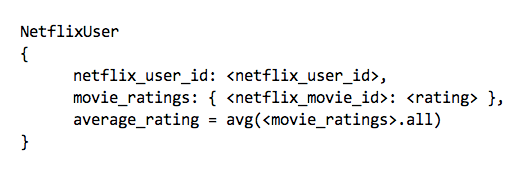
\includegraphics[width=4in]{image/datastructure-netflix-user.png}
	\centering
	\caption{The implemented datastructure of a NetflixUser. Curly brackets denote a hash. Square brackets denote a list of items of a certain type. Text encapsulated in smaller than bigger than denotes keys in the object it is declared in or other objects. Black keys are required, while grey keys are not required.}
	\label{figure:datastructure-netflix-user}
	\end{figure}

\subsubsection{Movie}
The NetflixUser datastructure models the movies in the netflix prize dataset. The implementation have the keys title and year which reflects the title of the movie and the year it was released. It also reflects the netflix users that have rated the movie and the rating itself. The implementation can be seen in figure~\ref{figure:datastructure-netflix-movie}.

	\begin{figure}[H]
	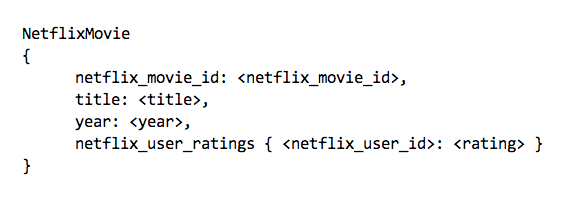
\includegraphics[width=4in]{image/datastructure-netflix-movie.png}
	\centering
	\caption{The implemented datastructure of a NetflixMovie. Curly brackets denote a hash. Square brackets denote a list of items of a certain type. Text encapsulated in smaller than bigger than denotes keys in the object it is declared in or other objects. Black keys are required, while grey keys are not required.}
	\label{figure:datastructure-netflix-movie}
	\end{figure}

\subsection{Data structure: Twitter}

\subsubsection{User}
The TwitterUser datastructure models users harvested from Twitter. The implementation have the key name which reflects the users nickname on Twitter. It also reflects the optional many relationship to TwitterTweets which referes to a collection of Tweets posted by the user. The TwitterUser's relationship to other TwitterUsers are reflected in the optional many relationships followees and followers. The key related\_to\_netflix\_movie refers to which NetflixMovie the user was harvested and is a Twitter data point for. The implementation can be seen in figure~\ref{figure:datastructure-twitter-user}.

	\begin{figure}[H]
	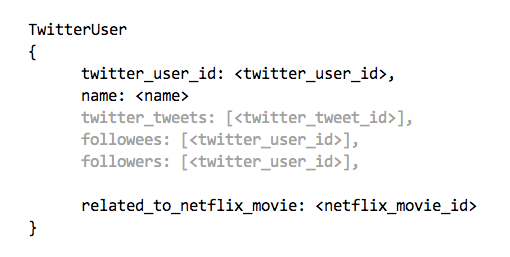
\includegraphics[width=4in]{image/datastructure-twitter-user.png}
	\centering
	\caption{The implemented datastructure of a TwitterUser. Curly brackets denote a hash. Square brackets denote a list of items of a certain type. Text encapsulated in smaller than bigger than denotes keys in the object it is declared in or other objects. Black keys are required, while grey keys are not required.}
	\label{figure:datastructure-twitter-user}
	\end{figure}

\subsubsection{Tweet}
The TwitterUser datastructure models tweets harvested from Twitter. The implementation have the key text which reflects the text content of the Tweet, and the key by\_twitter\_user which reflects which user posted the tweet. The key related\_to\_netflix\_movie refers to which NetflixMovie the user was harvested and is a Twitter data point for. The implementation can be seen in figure~\ref{figure:datastructure-twitter-user}.

	\begin{figure}[H]
	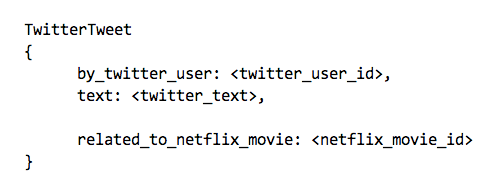
\includegraphics[width=4in]{image/datastructure-twitter-tweet.png}
	\centering
	\caption{The implemented datastructure of a TwitterTweet. Curly brackets denote a hash. Square brackets denote a list of items of a certain type. Text encapsulated in smaller than bigger than denotes keys in the object it is declared in or other objects. Black keys are required, while grey keys are not required.}
	\label{figure:datastructure-twitter-user}
	\end{figure}

\subsection{Data structure: Dataset}
This datastructure is not implemented due to the fact that it is only needed by the dataset building algorithm in section~\ref{algorithm-design:dataset-building} which is not implemented.
\subsection{Data structure: Prediction}
This datastructure is not implemented due to the fact that it is only needed by the prediction algorithm in section~\ref{algorithm-design:prediction} which is not implemented.

\section{Functional Modules}\label{impl:Functional Modules}

\subsection{Fields}
\subsubsection{Scrape}
Scrape is implemented using Anemone, a ruby gem that does event based crawling. Anemone is initialized with a url. It then retrieves the first page and extracts the urls from this page and append them to the crawler queue. It then initializes up to 4 threads that each grab urls from the crawler queue. It crawls the url and adds the pages to the page queue as they come in. When the last page is popped from the page queue without any new urls to crawl, Anemone finishes.

In the implementation, Anemone is initialized with a Twitter search query, like in Search Request in section~\ref{sec:pre-twitter-crawl-scrape}
The primary events in Anemone that are used by scrape follow.

	\begin{itemize}
	\item on\_every\_page
	\item focus\_crawl
	\item after\_crawl
	\end{itemize}

The event on\_every\_page is triggered every time Anemone extracts a page from the page queue. The process passed to this event gets the page as a Nokogiri page. Nokogiri is a ruby gem for parsing XML. The knowledge of the structure of the search result page from the prestudy in section~\ref{sec:pre-twitter-crawl-scrape} is used together with XPATH in Nokogiri to retrieve a list of TwitterTweets from the page. The TwitterTweets are stored in mongoDB automatically with MongoMapper.

The event focus\_crawl is triggered after every page and is responsible for delivering the list of URLs to anemone that should be put in the crawler queue. The scroll cursor and scroll cursor URL mentioned in section~\ref{sec:pre-twitter-crawl-scrape} under Scroll Search Results is retrieved from the page and pushed to the crawler queue. If there is no scroll cursor, Scrape prompts the harvester for another item to generate an initial search url for a new item.

The event after\_crawl is triggered after no more urls can be generated. This should not happen unless the harvester has no more items that should be crawled. However, in something goes wrong, the event asks the harvester for a new item and keeps crawling.

\subsubsection{Stream}
Stream is implemented separately from the twilm projects due to quicker development iteration. It is based on the gem tweetstream which is a full implementation of the Twitter Stream API. It connects to Twitter with OAuth for Twilm and the personal Twitter user account of one of the authors. The OAuth details are hardcoded into the application.

Stream is initialized by a harvester with a list of keywords. The keyword list retrieves all tweets that contain one or more of the keywords. The key to using Stream correctly is to define the keywords so that they return a set where the tweets wanted are a subset of this set. For netflix movies, this could be either one of the following

	\begin{itemize}
	\item movie
	\item film
	\item (list of all release years)
	\end{itemize}

\subsubsection{Search}
Search is similar but inferior to Stream, as discussed in section~\ref{sec:prestrud-eval-twitter}. It is therefore not implemented.

\subsubsection{REST}
REST is implemented using the ruby gem twitter. This gem is a full implementation of the Twitter REST API.

REST is contacted by a harvester to retrieve an item. The requests are functions defined in the fields class as follows.

	\begin{itemize}
	\item function followees(TwitterUser) returns [TwitterUser]
	\item function followers(TwitterUser) returns [TwitterUser]
	\item function twitter\_user(twitter\_user\_id) returns TwitterUser
	\item function tweets(TwitterUser) returns [TwitterTweets]
	\end{itemize}

Once an object has been retrieved from the Twitter REST API it is returned to the harvester that made the call to the function.

\subsection{Harvesters}
\subsubsection{HarvestTwitterTweetForNetflixMoviesWithScrape}
HarvestTwitterTweetForNetflixMovieWithScrape uses the field Scrape to harvest TwitterTweets related to all NetflixMovies. It iterates over NetFlixMovie.all. For the first NetflixMovie, it calls Scrape. The rest of the list is bound to a call back function next\_item\_to\_scrape. Scrape then knows to call this function to retrieve the next item when it is done with each item.

\subsubsection{HarvestFolloweesForTwitterUsersWithREST}
HarvestFolloweesForTwitterUsersWithREST uses the field REST to harvest followees for all TwitterUsers. It iterates over TwitterUser.all. For each TwitterUser, REST.followees(TwitterUser) is called. The list returned is merged with TwitterUser.followees and TwitterUser is saved.


\section{Testing}\label{impl:Testing}
\subsection{Data Structures}
The data structures were tested by creating, saving and cross checking with the database that they were being saved correctly. No formal unit testing was employed as the structures were fairly simple in structure to the point where formal test would only be testing the underlying technology. The following steps were taken to test the data structures.

	\begin{itemize}
	\item Create instances of each structures
	\item Save instance
	\item Confirm with mongoDB console
	\end{itemize}

First, an instance of each data structure with all the valid fields filled out correctly was first created. For example TwitterTweet. The lack of errors confirmed that the instances were created correctly.

Then, the instance was then saved using mongomappers document function save! which updates mongoDB with the document reflected in the object.

At last, the mongoDB console was opened and a query was made to make sure that the object had been created. Each field was then cross checked with the keys of the corresponding data structure instance to make sure they all matched.

\subsection{Fields}
The fields were tested by creating each field, calling the retrieval functions and making sure the retrieved items stored correctly in mongoDB. No formal functional testing was employed as the fields were fairly simple in functionality to the point where formal test would only be testing the underlying technology. The following steps were taken to test the fields.

	\begin{itemize}
	\item Create instances of each field
	\item Run functions available to harvester
	\item Confirm that a valid models returned and saved
	\end{itemize}

First, an instance of each field was created in order to make sure that the fields could be created properly and connect to their APIs without complications. An example would be "rest = REST.new", which would create an instance of the field REST.

Then, all the functions in the field available to the harvester for retrieving Twitter data points were run in order to see that they were returning valid TwitterTweets or TwitterUsers. An example would be calling rest.followees(some\_twitter\_user) and see if it returned a list of TwitterUsers.

At last, the Twitter data points returned by each function was saved by calling save! on each of them. Queries for mongoDB were then constructed to retrieve these items from the database. The items returned were then cross checked to see that they matched the data in each of the Twitter data points.

\subsection{Harvesters}
The harvesters were tested by creating the harvesters and making sure that they were storing the items that they retrieved in the database. No formal functional testing was employed as the harvesters were fairly simple in functionality to the point where formal test would only be testing the underlying technology. The following steps were taken to test the harvesters.

	\begin{itemize}
	\item Create instances of harvesters
	\item Output each item retrieved to the console
	\item Confirm with mongoDB console that models stored
	\end{itemize}

First, an instance of each harvester was created to make sure that there weren't any initialization errors. An example of this is "harvester = HarvestFolloweesForTwitterUsersWithREST.new"

Then, test code would print each item retrieved to the console. For the example, each item retrieved would be a list of TwitterUsers.

At last, mongoDB console queries were made to retrieve these items from the database to make sure that all objects were stored by the harvester and that the objects were the same.

\subsection{Not tested}
Testing of the RMSE score of the system is not tested since the needed data was not acquired from twitter~\ref{sec:twitter}, neither is the merging of the Netflix Prize dataset with the Twitter-data for the same reason, which is the dataset building from the requirement in~\ref{subsec:FR6}.

\subsubsection{The code}
The testing of implemented code is not done. This is because the implemented code is of such a nature that the extra work to produce the testing would be rendered redundant in comparison with the gain from the actual testing.
